\documentclass{beamer}
\mode<presentation> {
\usetheme{Boadilla}
\setbeamercovered{invisible}
\setbeamertemplate{navigation symbols}{} 
}

%\newcommand{\abs}[1]{\ensuremath{\left|#1\right|}}
%\newcommand{\bracket}[2]{\ensuremath{\left\langle#1 \vphantom{#2}\middle|  #2 \vphantom{#1}\right\rangle}}

\usepackage{amsmath, amsfonts, amssymb}
\usepackage{graphicx}
\title[HCA]{Hierarchical Controller Architecture for SDN}
\author[]{\textbf{Gourav Khaneja\\Sweta Yamini Seethamraju} \\ \small{Supervisor:} Prof. Philip Brighten Godfrey}
\date{\today}

\begin{document}
\frame{
\titlepage
}

\frame{
\frametitle{Outline}
\tableofcontents
}

\section{Introduction and Related Work}

\frame{
\frametitle{Problem}
\begin{itemize}
	\item Single controller architecture is not scalable
	\item Distributed controller architectures provide global view to control application
\pause
	\item Problems are
	\begin{itemize}
		\item Communication overhead
		\item Network state inconsistencies
		\item Management barriers across networks 
		\item Scalability of complete global view of the network
	\end{itemize}
\pause
	\item Trade-offs
	\begin{itemize}
		\item Consistency vs. Responsiveness
		\item Application design complexity (architecture aware vs. agnostic)
	\end{itemize}
\pause
	\item Aim
	\begin{itemize}
		\item Make control application agnostic to underlying distributed architecture
		\item Aggregate network to simplify network view
		\item Handle inconsistency in "SDN datapath"
	\end{itemize}
\end{itemize}
}

\frame{
\frametitle{Previous Work}
\begin{itemize}
	\item Hyperflow
\pause
	\begin{itemize}
		\item Flat distributed controller architecture
		\item Applications are agnostic to underlying state distribution
		\item Provides a logically centralized global view of the network
		\item Results in performance degradation and transient inconsistencies
	\end{itemize}
\pause
	\item Onix
\pause
	\begin{itemize}
		\item Provides flexible framework to handle controller topology
		\item Provides generic distributed state management API
		\item Provides a framework but not an approach
		\item Design decisions left to control application
	\end{itemize}
\pause
	\item Kandoo
\pause
	\begin{itemize}
		\item Two-level controller architecture
		\item Events are propagated only on subscription
		\item Applications need to be aware of hierarchy
		\item View of root controller varies with control application
	\end{itemize}
\end{itemize}
}

\section{Approach and Progress}

\frame{
\frametitle{Our Approach}
\begin{itemize}
\item What is being done ? 
	\begin{itemize}
		\item It's a Replicated state machine (strong or lazy replication) architecture, which had been well studied in Distributed Systems community
		\item Past work uses DHTs (Onix), Transactional DB (Onix), DFS (Hyperflow)
	\end{itemize}
	\item We are trying to study		
	\begin{itemize}
		\item Instead of just using a general replication mechanism, can we exploit the fact that network views are being replicated ?
		\item Could SDN datapath (replication client) make use of replication timestamps ?
	\end{itemize}
	
	
\end{itemize}
}

\frame{
\frametitle{Hierarchical Architecture}
\begin{itemize}
	\item Controllers' view do not span the whole network, but only the 'underlying network'
	\item A controller behaves as an openflow switch for parent controller (Network Aggregation) and as a controller for its underlying network
	\item Controller translates OFP commands and network updates between parent controller and underlying networks
	\item Control applications run on each controller to set the network parameters in its underlying network
\end{itemize}
}

\frame{
\frametitle{Simulation}
\begin{itemize}
	\item Wrote a simulator to simulate a hierarchical controller architecture\footnote{code @ https://github.com/MugiwaraLuffy/ACN/tree/master/simulator/src/swiconsim}
	\item A minimal set of APIs for control plane, data plane, controller behavior, etc has been defined
	\item A $Node$ is an element in the management network which implements $IControlPlane$ interface 
	\item A $Switch$ extends a $Node$ and contains a data plane
	\item A $Controller$ extends a $Node$ and implements standard controller APIs
	\item $DataNetwork$ contains all the switches which handle actual data packets
	\item A $Controller$ controls a $Node$ which could be a $Switch$ or another $Controller$
\end{itemize}
}

\frame{
\frametitle{Network Aggregation}
	\begin{itemize}		
		\item Definition - Create and publish one flow table (referred to as $nflow$) for a given network. (1) Support addition of flows to $nflow$ efficiently. (2) Handle intra-link failure efficiently, in such a way that $nflow$  does not change.
		\item $nflow$ schema $(port in, flow in, port out, flow out, priority, attributes)$
		\item Data structures\footnote{code @ https://github.com/MugiwaraLuffy/ACN/tree/master/simulator/src/graph}:
		\begin{itemize}
			\item Add $external$ $nodes$ to the network graph $G$
			\item Flow graphs: For each external node, $e$, we create/maintain a directed flow graph, $f_e$ as an overlay graph on $G$, rooted at $e$, which is the source. End host and other external nodes acts as sink. The flow in $f_e$ are divided at nodes among the incident links according to the flow tables at corresponding routers.
			\item Other data structures include: Path array, Link array 
		\end{itemize} 		
	\end{itemize}
}

\frame{
\frametitle{Timestamp}
	\begin{itemize}
		\item An example - Link Balancer Controller [4]
		\item On a flow arriving at an ingress port, a path with minimum maximum utilization is chosen
		\item Each domain $i$ maintains a vector timestamp, $T_{i}[1...n]$. $T_{i}[j]$ contains the latest revision number of domain $j$ link utilizations, seen by domain $i$
		\item Each router in a domain is updated with domain's timestamp
		\item When a flow path is being set up at domain $j$, it is augmented by the $T_{j}$
		\item When a router in a domain $i$ receives a flow with timestamp $T_{j}$, it may change part of flow's path if $T_{j}[i] < T_{i}[i]$ 
		\item Flow's timestamp is updated as $max\{T_{j}[k], T_{i}[k]\}$ , $k=1...n$ 
		\item OK, can we do better ? Yes!, a domain can change the entire flow's path according to timestamps.
	\end{itemize}   
}

\frame{
\frametitle{Preliminary Results}
%\begin{itemize}
%\item Preliminary link utilization plots
%\end{itemize}
\begin{figure}
 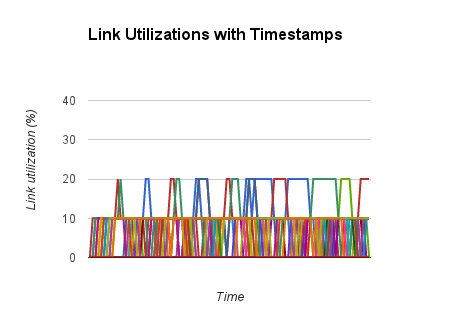
\includegraphics[scale=0.3]{chart_1}
 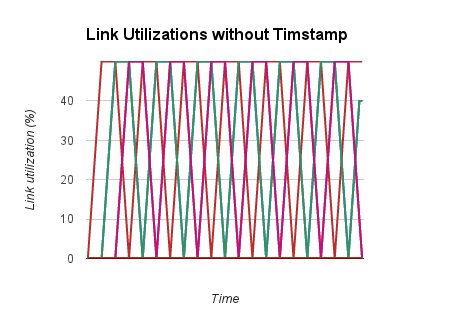
\includegraphics[scale=0.3]{chart_2}
\caption{Comparision of Link utilizations with/without Timestamp \footnote{ \scriptsize Simulator @ https://github.com/MugiwaraLuffy/ACN/tree/master/simulator/src/timestamp}}
\end{figure}

'Long lived flows' flow between domain 1 and domain 3 through domain 2. A link balancer control application runs on each controller

}

\section{What next ?}



\frame{
\frametitle{Hitches}
\begin{itemize}
	\item Hierarchical Architecture
	\begin{itemize}
		\item Suboptimal performance
	\end{itemize}
	\item Network Aggregation
	\begin{itemize}
		\item May backfire: single internal update may cause multiple updates in aggregated network 
	\end{itemize}
	\item Timestamps
	\begin{itemize}
		\item Not a true datapath technique
		\item Improve the performance of control applications, however, does not provide any guarantees
	\end{itemize}
\end{itemize}	
}

\frame{
\frametitle{Future Work}
\begin{itemize}
	\item Understand the trade-off between sub-optimality and frequency of updates, in case of hierarchical architecture
	\item Revise Network Aggregation data structures so as not to explode network updates
	\item Implement and simulate each approach on real ISP topology with real traffic data. Analyze performance
\end{itemize}
}

\frame{
\centerline{Thank you!}
}

\frame{
\frametitle{References}
\begin{itemize}
\item [1] T. Koponen, M. Casado, N. Gude, J. Stribling, L. Poutievski, M. Zhu, R. Ramanathan, Y. Iwata, H. Inoue, T. Hama, and S. Shenker. Onix: a distributed control platform for large-scale production networks. In Proceedings of the 9th USENIX OSDI conference , pages 1 - 6, 2010.
\item [2] A. Tootoonchian and Y. Ganjali. Hyperflow: a distributed control plane for openflow. In Proceedings of the 2010 INM conference, 2010.
\item [3] Soheil Hassas Yeganeh and Yashar Ganjali. Kandoo: a framework for efficient and scalable offloading of control applications. In Proc. 1st Workshop on Hot Topics in Software Defined Networking (HotSDN 2012), pages 19-24, New York, 2012. ACM Press. 
\item [4] D. Levin, A. Wundsam, B.Heller, N. Handigol, and A. Feldmann, Logically Centralized State Distribution Trade-offs in Software Defined Networks  in HotSDN, 2012. 
\end{itemize}
}

\frame{
\begin{itemize}
\frametitle{References}
\item [5] Stefan Schmid and Jukka Suomela, Exploiting Locality in Distributed SDN Control, in HotSDN, 2013. 
\item [6] Advait Dixit, Fang Hao, Sarit Mukherjee, T. V. Lakshman and Ramana Kompella, Towards an Elastic Distributed SDN Controller, in HotSDN, 2013.
\item [7] Nate Foster, Rob Harrison, Matthew L. Meola, Michael J. Freedman, Jennifer Rexford and David Walker, Frenetic: A High-Level Language for OpenFlow Networks. ACM PRESTO 2010.
\end{itemize}
}

\end{document} 
